\documentclass[11pt, notheorems]{beamer}
\usepackage[utf8]{inputenc}
\usepackage[croatian]{babel}
\usepackage[T1]{fontenc}
\usepackage{amsmath}
\usepackage{amsfonts}
\usepackage{amssymb}
\usepackage{graphicx}
\usepackage{fixmath}
\usepackage{booktabs}
\usepackage{caption}
%\usecolortheme[snowy]{owl}
\usetheme{metropolis}

\newtheorem{theorem}{Teorem}

\newcommand{\q}{\left}
\newcommand{\w}{\right}

\newcommand{\matr}[1]{\mathbold{#1}}
\newcommand{\prob}[1]{\operatorname{\mathbf{P} \q(#1\w)}}

\begin{document}
  \author{Lovre Mrčela}
  \title{Analiza vremenskih nizova zasnovana na kompleksnim mrežama}
  \subtitle{Diplomski rad}
  \institute{Sveučilište u Zagrebu \\
             Fakultet elektrotehnike i računarstva \\
             \textbf{Zavod za elektroničke sustave i obradbu informacija}}
  \date{\today}
  \setbeamertemplate{navigation symbols}{}

  \begin{frame}[plain]
  \maketitle
  \end{frame}

  \begin{frame}{Sadržaj}
    \setbeamertemplate{section in toc}[sections numbered]
    \tableofcontents[hideallsubsections]
  \end{frame}
  
  \section{Uvod}
  \begin{frame}
    \frametitle{Cilj rada}
    \begin{itemize}
    \item optimizacija portfelja
    \item unaprjeđenje postojećih metoda \alert{statističke arbitraže}
    \item modeliranje \emph{interakcija vrijednosnica} korištenjem \alert{kompleksnih mreža}
    \end{itemize}
  \end{frame}

  \begin{frame}
    \frametitle{Teorem o nearbitraži}
    \begin{theorem}
      Ako je u trenutku 0 vrijednost portfelja $V\q(0\w) = 0$, tada je u nearbitražnim okolnostima vjerojatnost $\prob{V\q(t\w) > 0} = 0$ za $t > 0$.
    \end{theorem}
  \end{frame}

  \begin{frame}
    \frametitle{Koeficijent obrtaja}
    \begin{itemize}
      \item \emph{mjera promjenljivosti} portfelja
      \item u rasponu $\q[0, 2\w]$
      \item portfelj s $N$ vrijednosnica $\matr{\alpha} = \begin{bmatrix} \alpha_1 & \alpha_2 & \cdots & \alpha_N \end{bmatrix}$
      \item \alert{koeficijent obrtaja} $\eta^{(t)}$:
      \begin{equation*}
        \eta^{(t)} = \sum_{i=1}^{N} \q \lvert \alpha_i^{(t)} - \alpha_i^{(t-1)} \w \rvert
      \end{equation*}
      \item \emph{veći koeficijent obrtaja --- veći troškovi trgovanja}
    \end{itemize}
  \end{frame}
  
  \section{Statistička arbitraža}
  \begin{frame}
    \frametitle{Metoda}
    \only<1>{
    Okvir postupka statističke arbitraže:
    \begin{enumerate}
      \item identificirati parove vrijednosnica čije cijene se \emph{slično ponašaju}
      \item među tim parovima izdvojiti one kod kojih je utvrđeno \emph{statistički značajno odstupanje}
      \item svaki izdvojeni par \emph{uvrstiti u portfelj}, odnosno zauzeti \alert{kratku} i \alert{dugu} poziciju; jednom kada odstupanje prestane, \emph{zatvoriti otvorene pozicije}
    \end{enumerate}}
    \only<2>{
     \begin{figure}
       \centering
       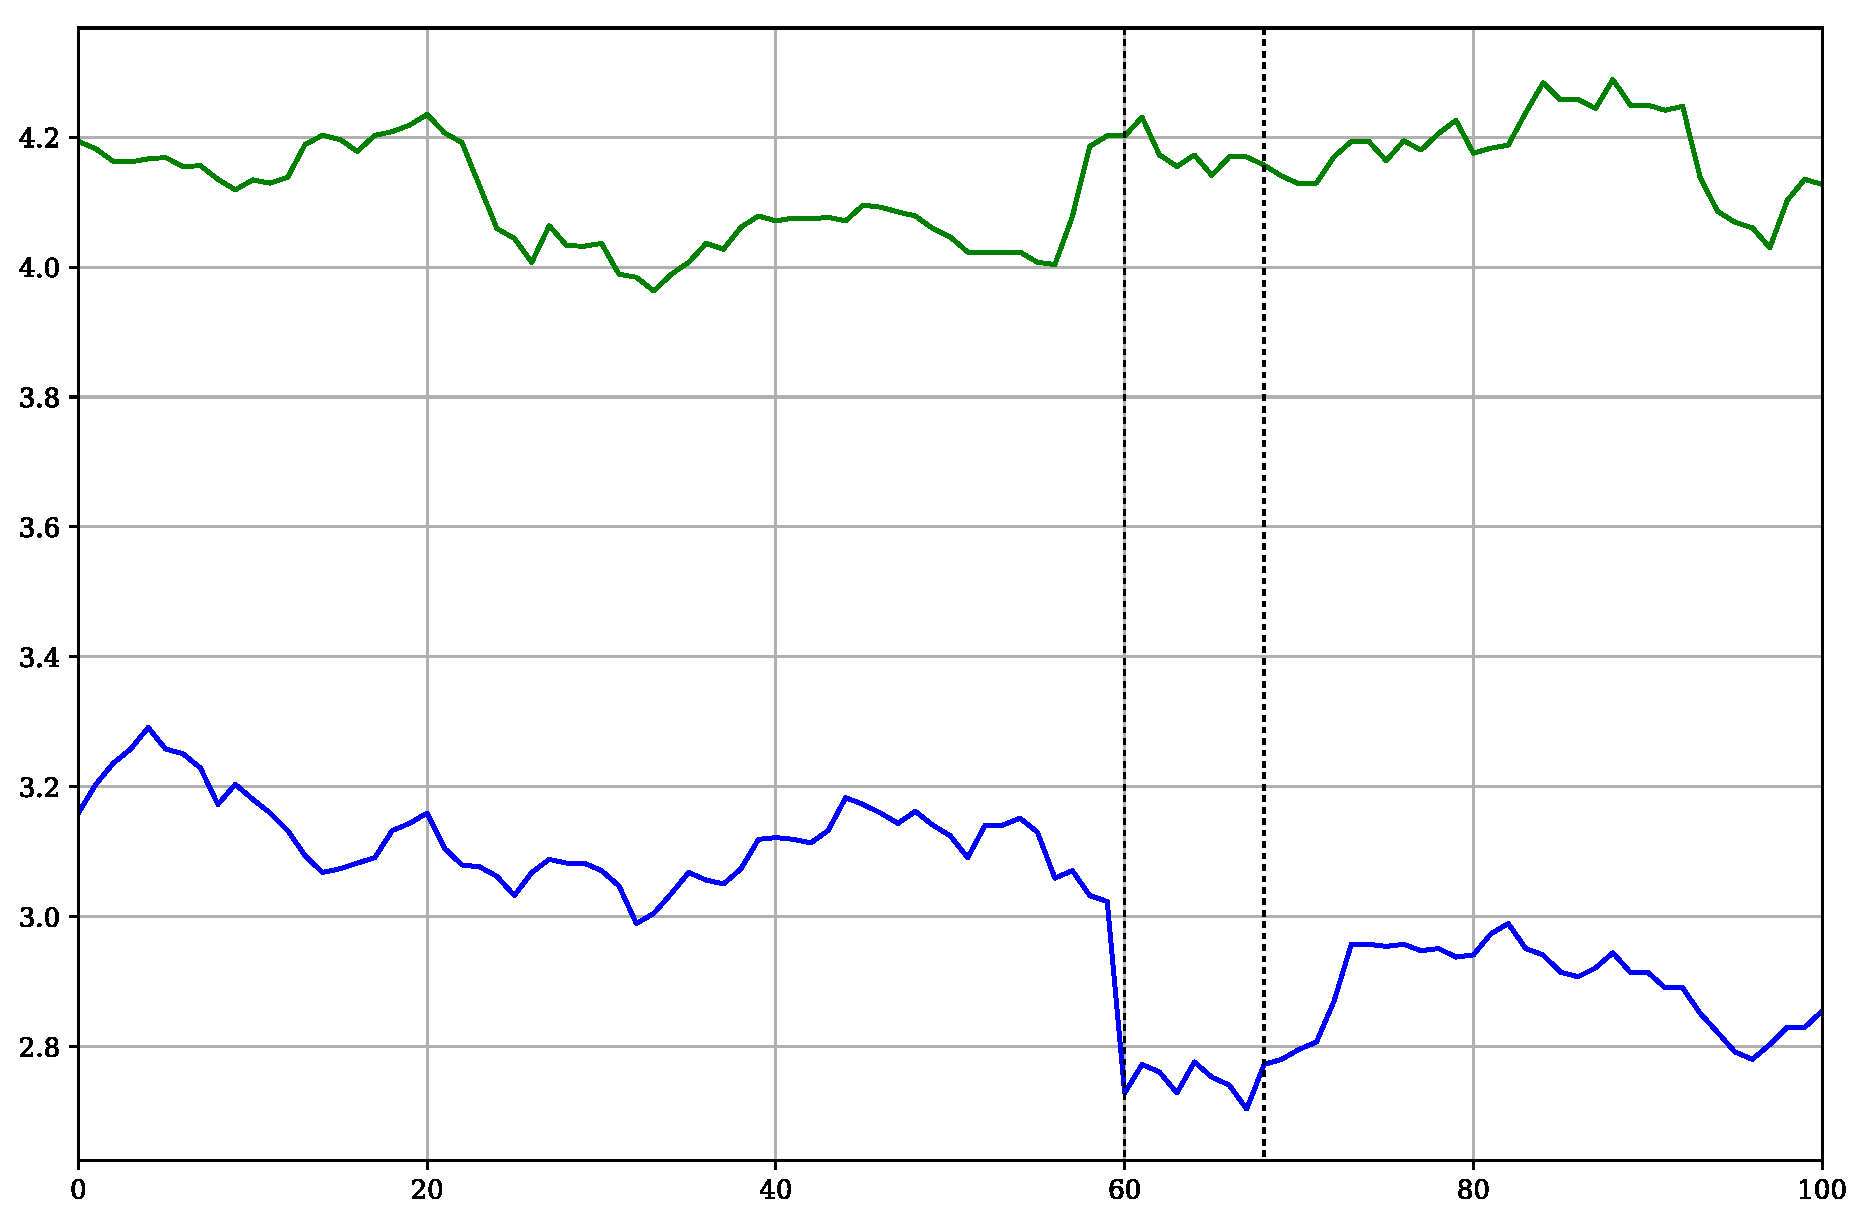
\includegraphics[width=\textwidth]{graphics/trading-signal.pdf}
       \caption*{Kretanje cijena dviju vrijednosnica.}
     \end{figure}}
     \only<3>{
       \begin{figure}
         \centering
         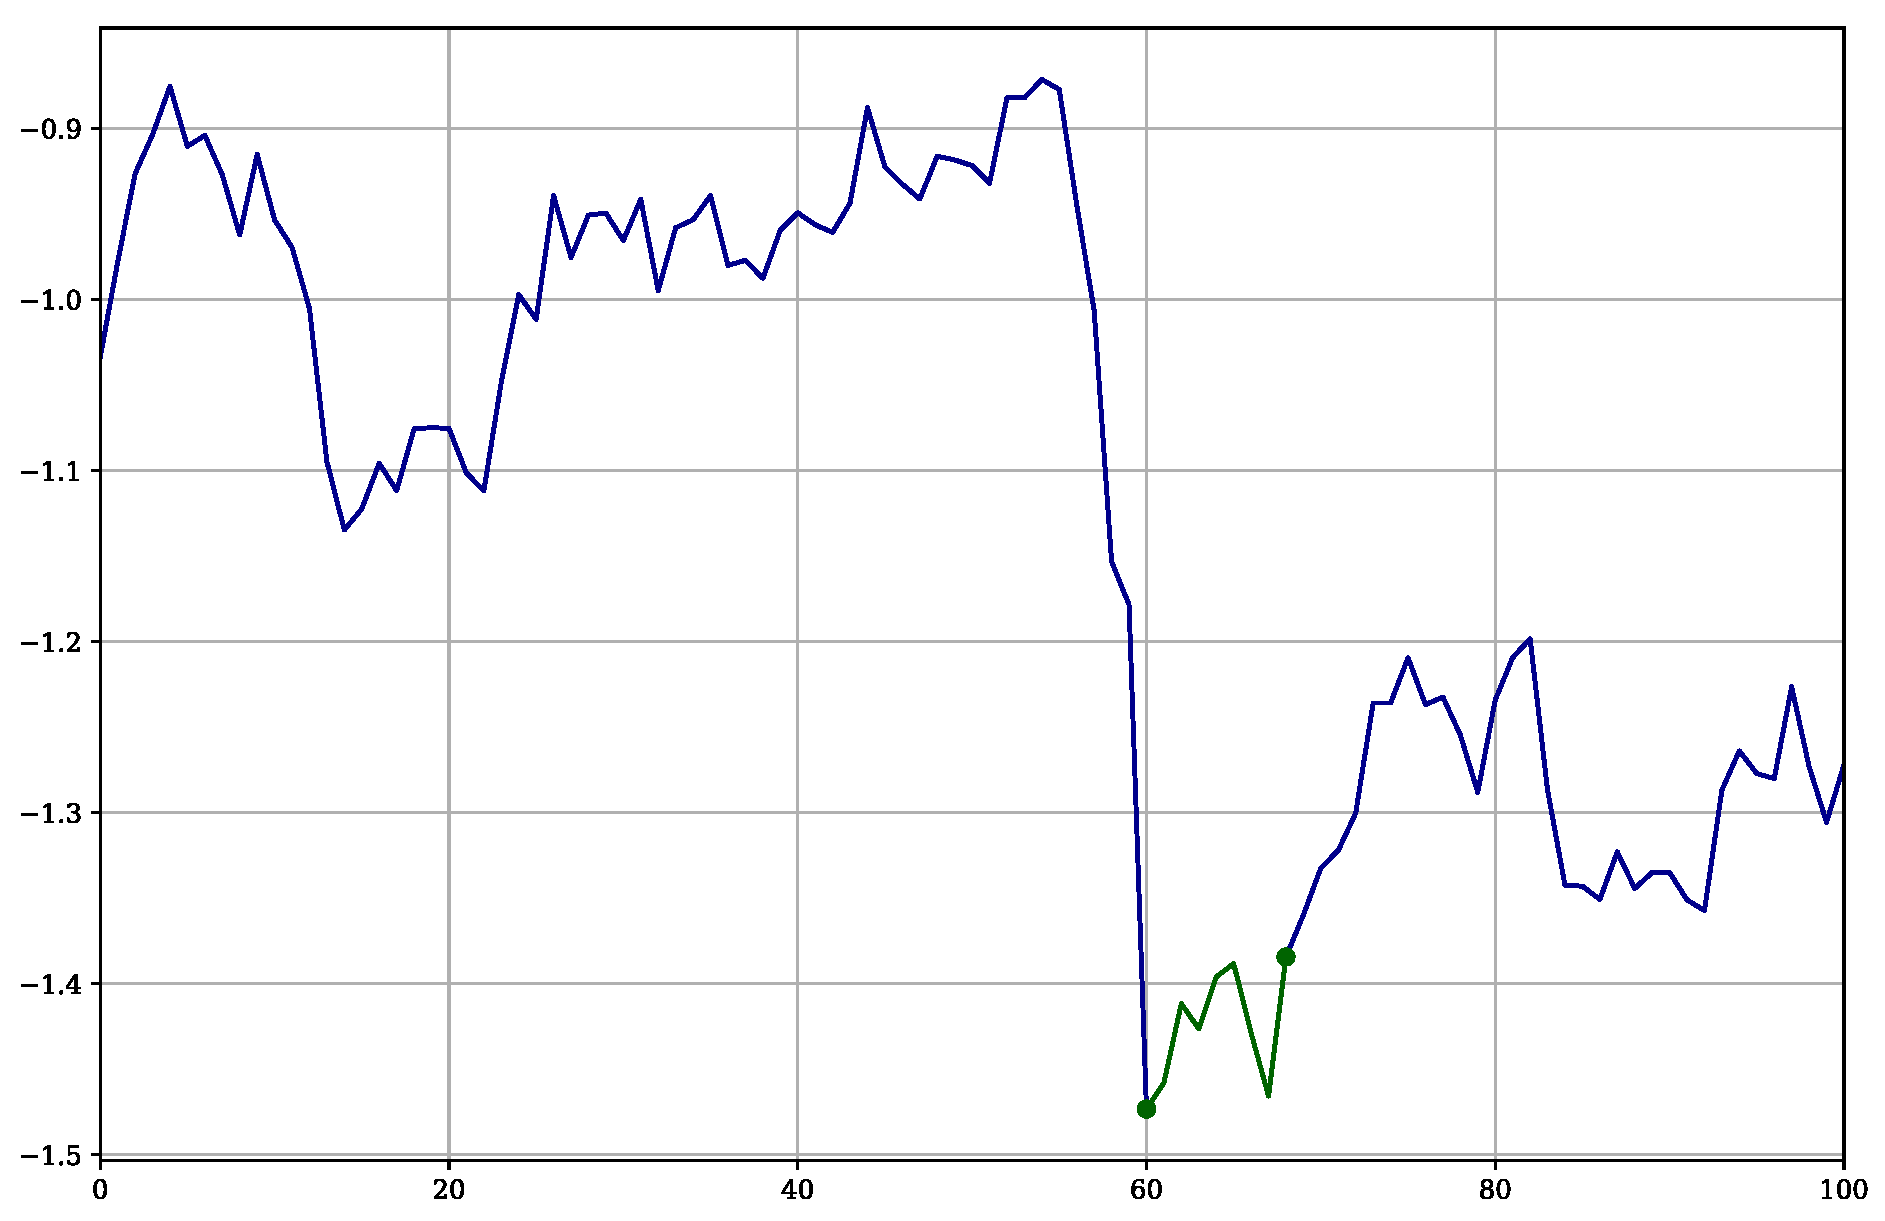
\includegraphics[width=\textwidth]{graphics/trading-diffs.pdf}
         \caption*{Razlika cijena istih dviju vrijednosnica.}
     \end{figure}}
  \end{frame}

  \begin{frame}
    \frametitle{Signal trgovanja}
    \only<1>{
      \begin{gather*}
      c_{i,j} \text{ --- razlika logaritamskih cijena vrijednosnica } i \text{ i } j \\
      m_{i,j}^{\q(t\w)} = \frac{1}{T}\sum_{\tau = t - T}^{t - 1} c_{i,j}^{(\tau)} \\
      d_{i,j}^{\q(t\w)} = \sqrt{\frac{1}{T - 1}\sum_{\tau=t - T}^{t - 1} \q(c_{i,j}^{(\tau)} - m_{i,j}^{\q(t\w)} \w)^2} \\
      \Gamma_{X, Y}^{(t)} = \frac{c_{X,Y}^{
          \q(t\w)} - m_{X,Y}^{\q(t\w)}}{d_{X,Y}^{\q(t\w)}}
      \end{gather*}
    }
    \only<2>{
    \begin{figure}
      \centering
      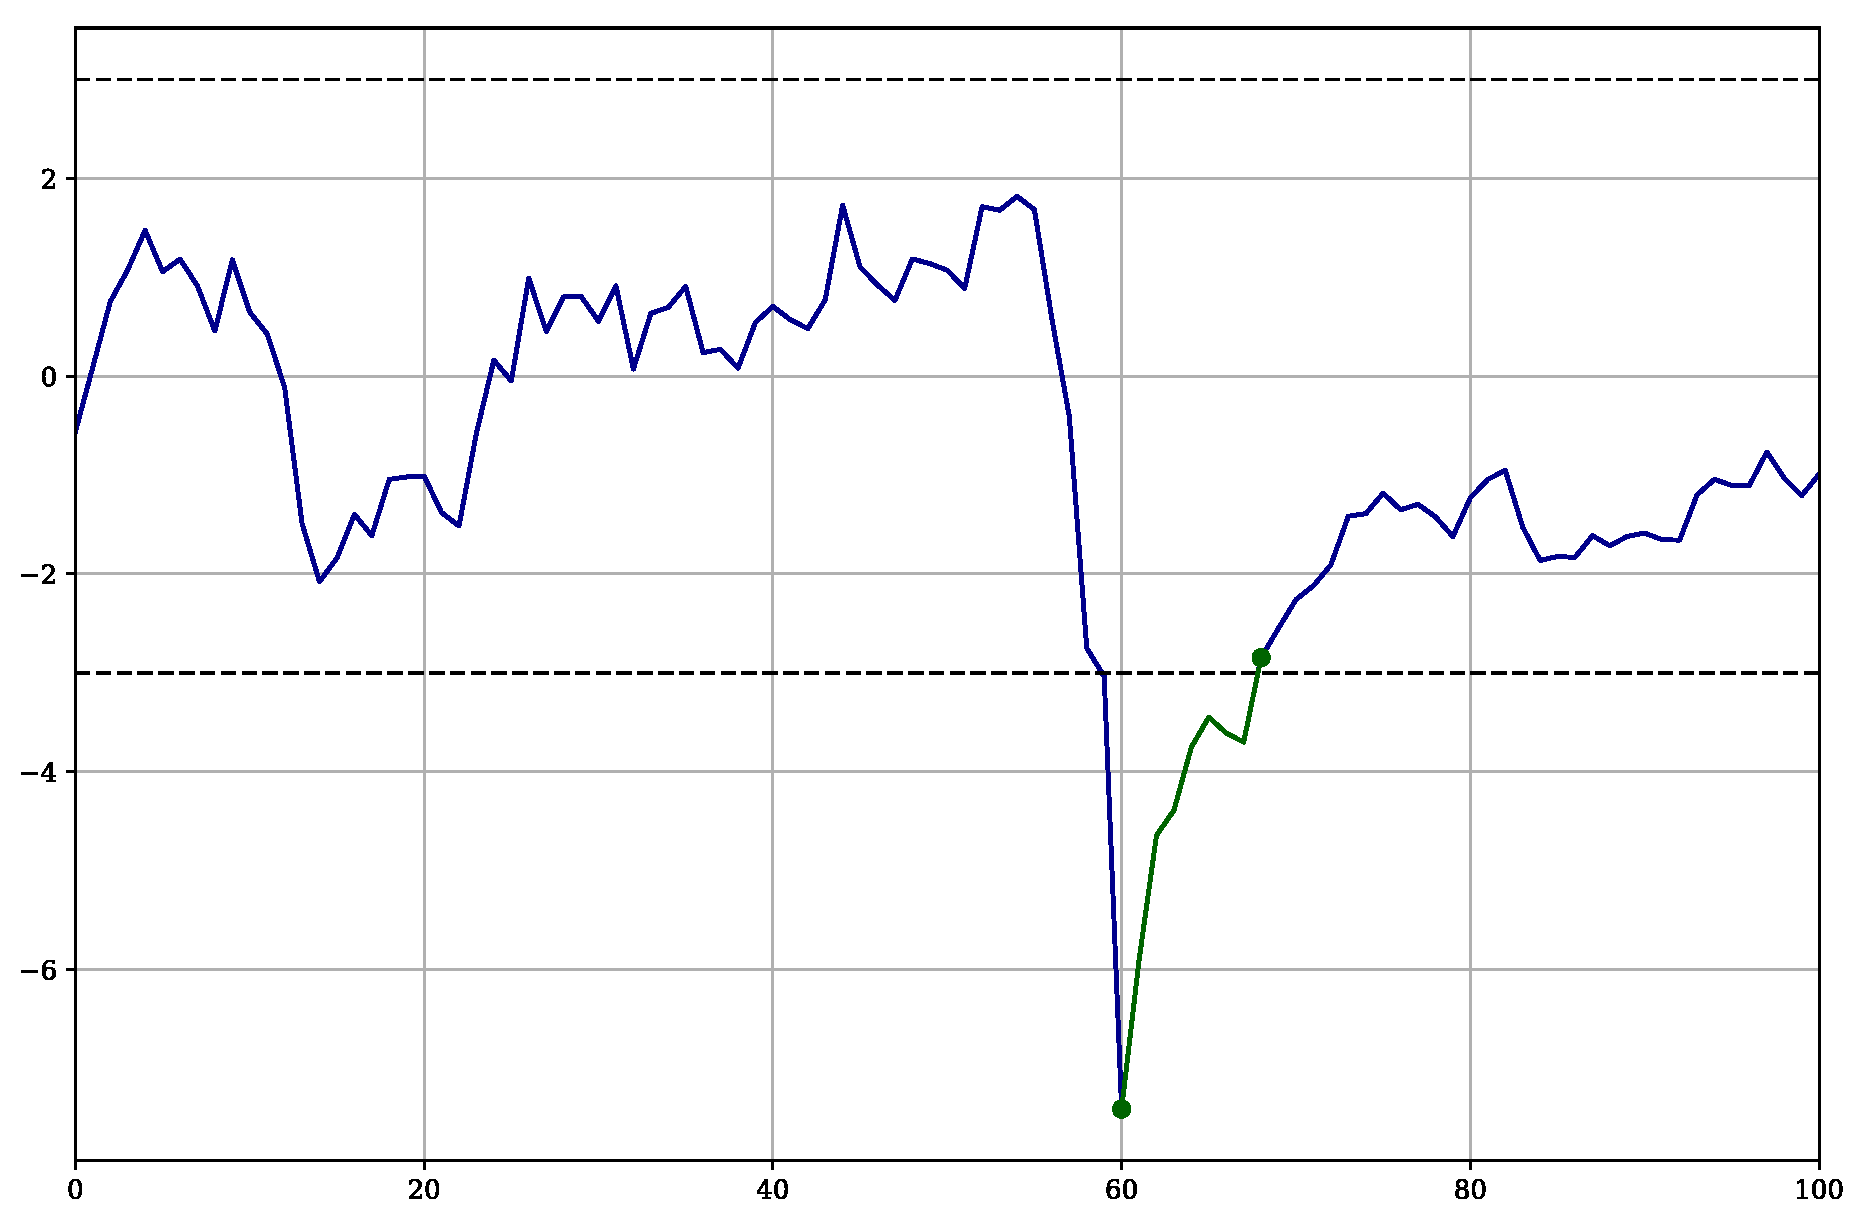
\includegraphics[width=\textwidth]{graphics/trading-prices.pdf}
      \caption*{Signal trgovanja dobiven iz istih dviju vrijednosnica.}
    \end{figure}}
  \end{frame}

  \begin{frame}
    \frametitle{Nedostaci}
    \begin{itemize}
      \item preciznost rijetko kada \textbf{iznad 60\%}, u većini slučajeva \textbf{manja od 50\%}
      \item trgovanje u parovima, zahtijeva mogućnost zauzimanja \alert{kratke pozicije}
      \item velika promjenljivost portfelja, \alert{visoki troškovi trgovanja}
    \end{itemize}
  \end{frame}

  \section{Tok preferencija}
  \begin{frame}
    \frametitle{Relacija preferencije}
    \begin{itemize}
      \item \textbf{binarna relacija:} $a \succ b$ --- $a$ je \emph{više preferirano} od $b$
      \item \emph{indiferentnost} u izboru: $a \sim b$ --- $a$ \emph{nije usporedivo} s $b$
      \item \emph{ljudski} način uspoređivanja dobara
      \item \emph{irefleksivna}, \emph{asimetrična}, \emph{tranzitivna}, i \emph{tranzitivna po indiferentnosti} 
    \end{itemize}
  \end{frame}

  \begin{frame}
    \frametitle{Graf toka preferencija}
    \only<1>{
    \begin{itemize}
      \item \alert{relacija preferencije} ne definira \emph{poredak} dobara, nema \emph{intenzitete} preferencije
      \item \alert{graf toka preferencija} uvodi \emph{intenzitete} preferencije, modelira \emph{interakciju} vrijednosnica
      \item pomoćna struktura
      \item ne mora biti \alert{konzistentan}
    \end{itemize}}
    \only<2>{
      \begin{figure}
        \centering
        \begin{minipage}{0.45\textwidth}
          \centering
          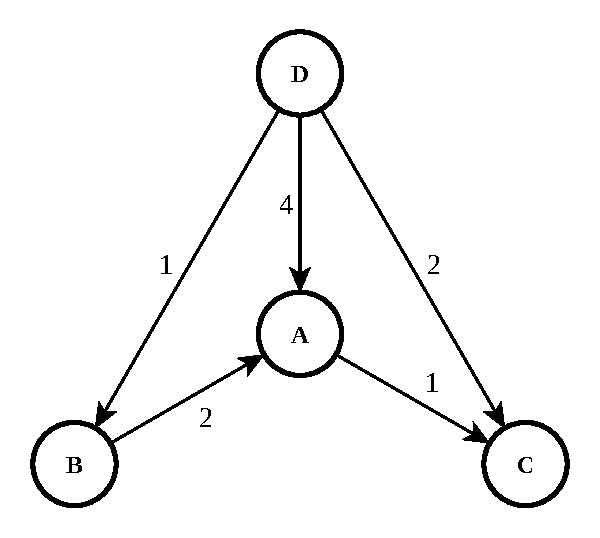
\includegraphics[width=0.808\textwidth]{graphics/graph-eg-1.pdf}
          \caption*{Nekonzistentan graf.}
        \end{minipage}
        \hfill
        \begin{minipage}{0.45\textwidth}
          \centering
          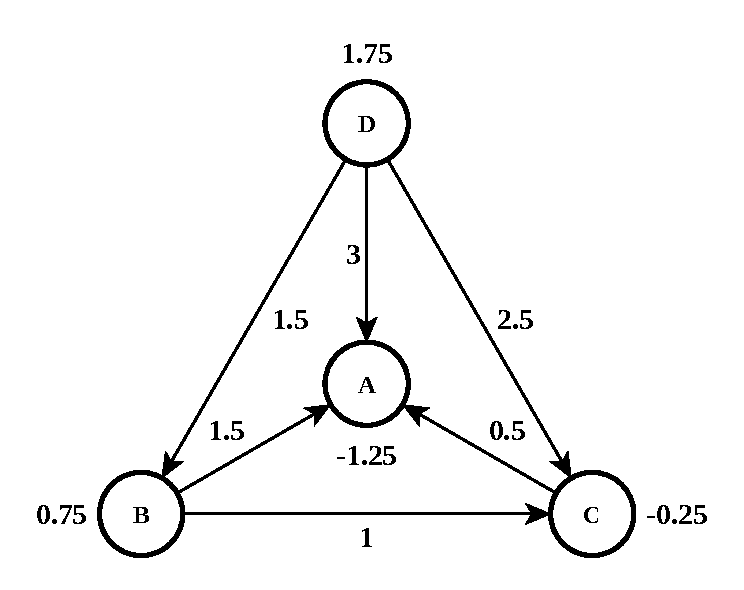
\includegraphics[width=\textwidth]{graphics/graph-eg-2.pdf}
          \caption*{Konzistentan graf.}
        \end{minipage}
      \end{figure}}
  \end{frame}

  \begin{frame}
    \frametitle{Metoda potencijala}
    \only<1>{
    \begin{itemize}
      \item ni \alert{graf toka preferencija} ne definira \emph{poredak} dobara
      \item \alert{metoda potencijala} definira \emph{poredak} dobara na temelju grafa, i daje \alert{mjeru konzistentnosti} grafa, u rasponu $\q[0, 1\w]$
      \item \alert{mjera konzistentnosti} opisuje koliko je odluka donesena na temelju grafa \emph{pouzdana}
    \end{itemize}}
    \only<2>{
      \begin{figure}
        \centering
        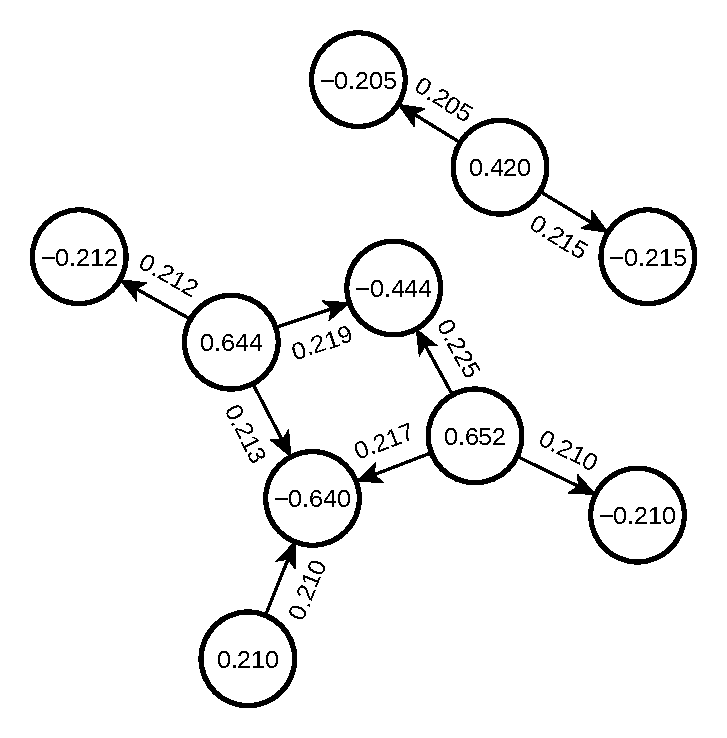
\includegraphics[width=0.6\textwidth]{graphics/pref-flow-graph.pdf}
        \caption*{Rezultat korištenja metode potencijala.}
      \end{figure}}
  \end{frame}

  \begin{frame}
    \frametitle{Cjelokupni algoritam trgovanja}
    \begin{enumerate}
      \item pomoću \emph{metode} \alert{statističke arbitraže} dobiju se \emph{opisi} \alert{toka preferencija} u grafu
      \item iz \alert{grafa toka preferencija} korištenjem \alert{metode potencijala} određuje se poredak vrijednosnica \emph{prema preferenciji}
      \item u vrijednosnicama s \textbf{najvećom} preferencijom zauzima se \textbf{duga} pozicija, a u onima s \textbf{najmanjom kratka} (ako je to dopušteno)
    \end{enumerate}
  \end{frame}

  \section{Praktični dio}
  \begin{frame}
    \frametitle{Implementacija}
    \begin{itemize}
      \item \alert{\textit{Python}} (\emph{NumPy}, \emph{pandas}, \emph{SciPy}, \emph{Matplotlib})
      \item \alert{\textit{Jupyter} bilježnica}
      \item \emph{open source} alati
      \item metoda statističke arbitraže i metoda potencijala
      \item skripte za simuliranje trgovanja
    \end{itemize}
  \end{frame}

  \begin{frame}
    \frametitle{Rezultati simulacija - S\&P 203}
    \only<1>{
    \begin{figure}
      \centering
      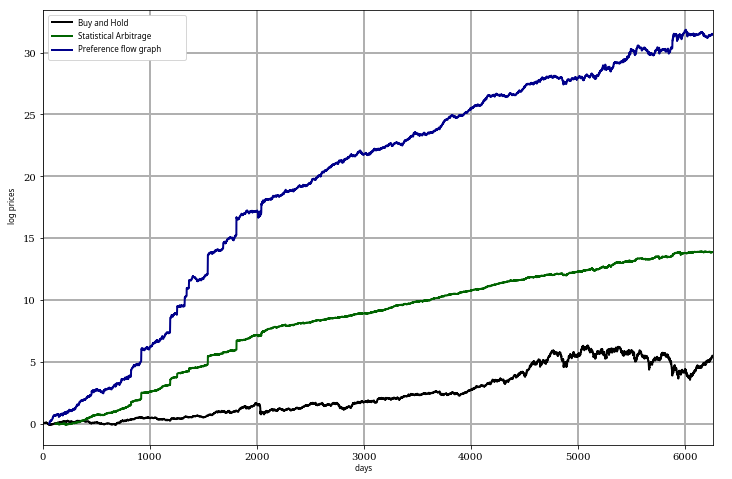
\includegraphics[width=\textwidth]{graphics/result1.png}
      \caption*{Rezultati simulacije na podskupu od 203 dionice iz S\&P 500.}
    \end{figure}}
    \only<2>{
      \begin{table}
        \centering
        \caption*{Rezultati simulacije na podskupu od 203 dionice iz S\&P 500.}
        \resizebox{\textwidth}{!}{\begin{tabular}{lrrr}
          \toprule
          \textbf{Metoda} & `Buy \& Hold' & Statistička arbitraža & Tok preferencija \\
          \midrule
          \textbf{Godišnji povrat} & 0.07622 & 0.63033 & \textbf{1.28000} \\
          \textbf{Volatilnost} & \textbf{0.15069} & 0.33532 & 0.78373 \\
          \textbf{Sharpeov omjer} & 0.50582 & \textbf{1.87981} & 1.63322 \\
          \textbf{Prosječni turnover} & / & 1.473211 & \textbf{0.55112} \\
          \midrule
          \textbf{Profit uz troškove trgovanja 0.10\%} & 5.49572 & $-2.74051$ & 24.66204 \\
          \bottomrule
        \end{tabular}}
      \end{table}}
\end{frame}

  \begin{frame}
    \frametitle{Rezultati simulacija - S\&P 500}
    \only<1>{
      \begin{figure}
        \centering
        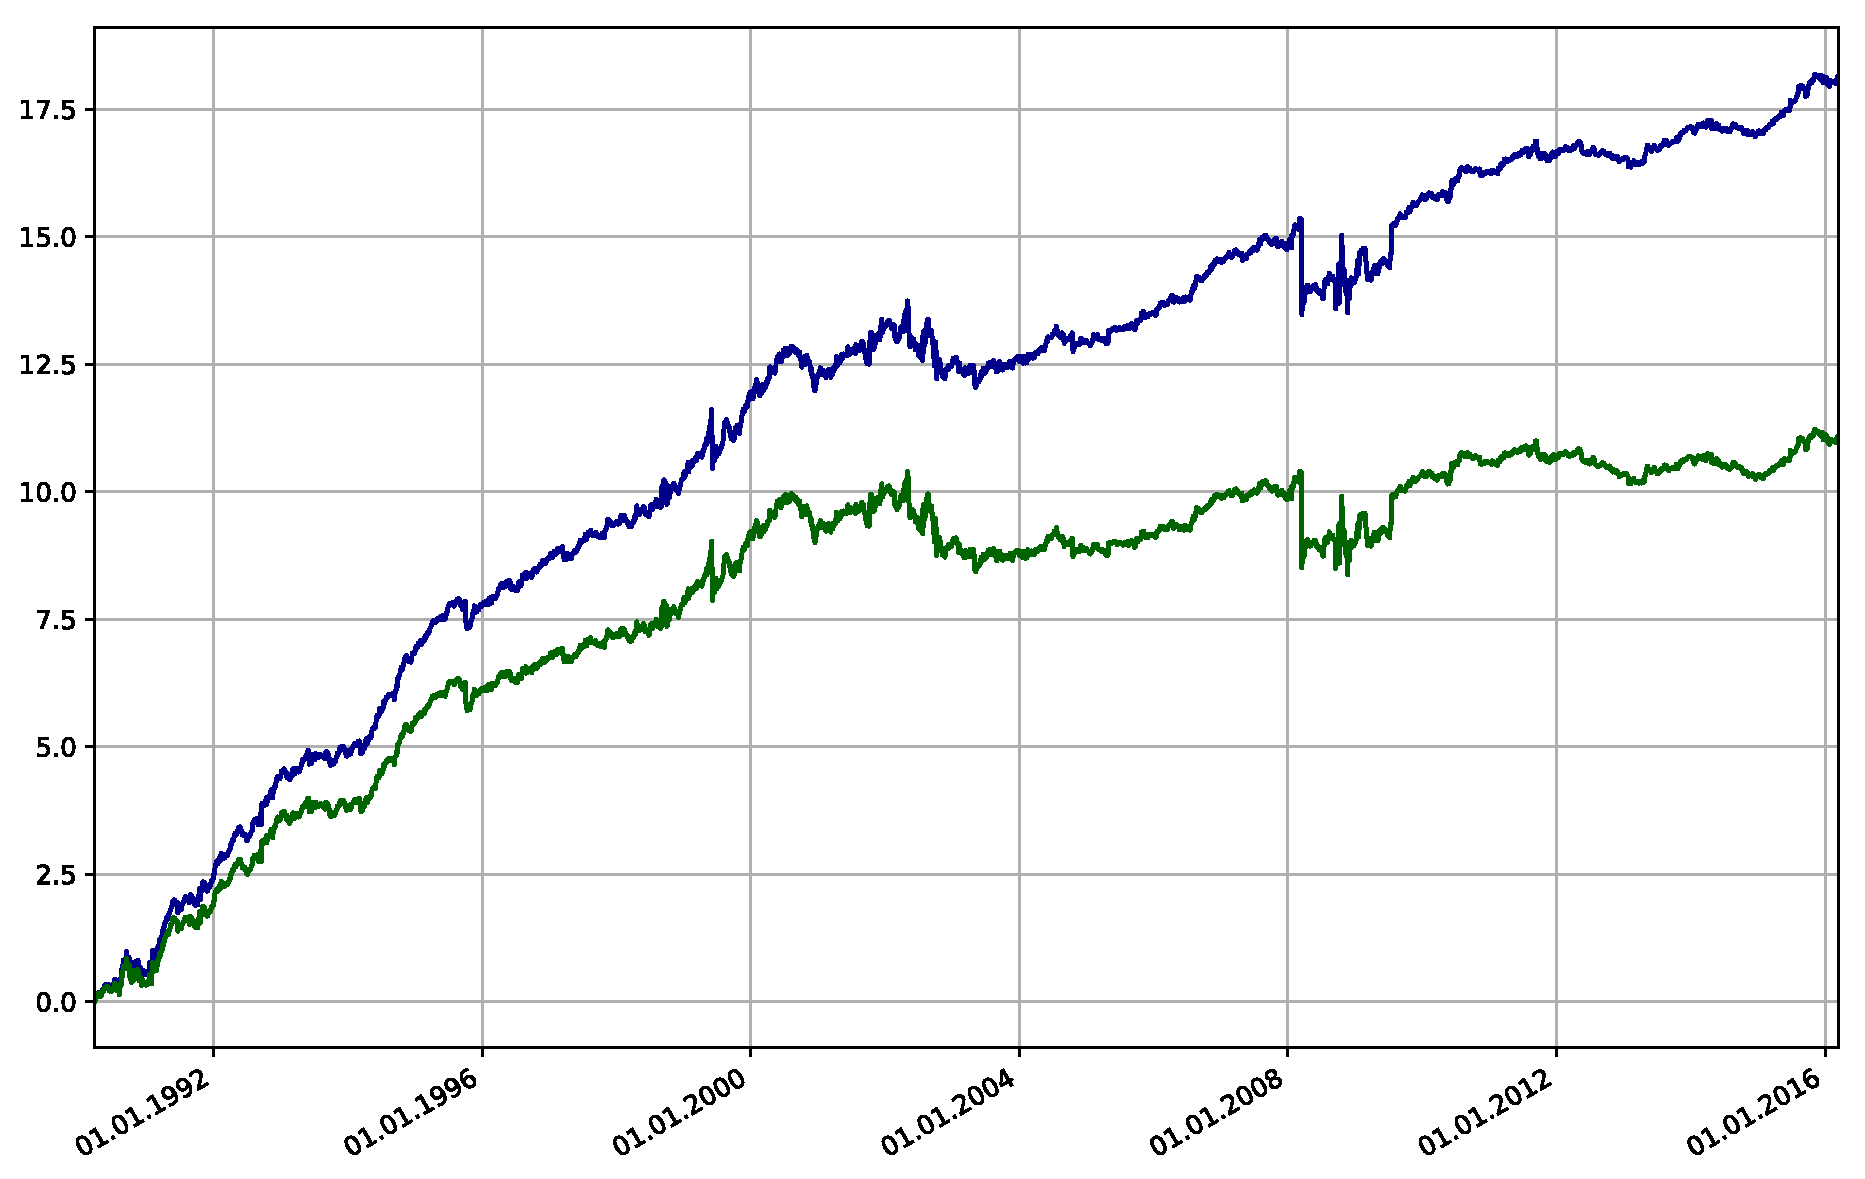
\includegraphics[width=\textwidth]{graphics/sp500full-profits.pdf}
        \caption*{Rezultati simulacije na punom skupu dionica iz S\&P 500.}
    \end{figure}}
    \only<2>{
      \begin{table}
        \centering
        \caption*{Rezultati simulacije na punom skupu dionica iz S\&P 500.}
        \resizebox{0.8\textwidth}{!}{\begin{tabular}{lr}
            \toprule
            Rezultati: & \\
            \midrule
            bez troškova trgovanja: & \\
            ukupni profit & 18.09261 \\
            Sharpeov omjer & 0.87507 \\
            \midrule
            {uz uključene troškove trgovanja od 0.10\%:} & \\
            ukupni profit & 11.03961 \\
            Sharpeov omjer & 0.53382 \\
            \midrule
            prosječni koeficijent obrtaja & 1.04088 \\
            prosječna konzistentnost & 0.55817 \\
            prosječna preciznost & 0.52642 \\
            \bottomrule
        \end{tabular}}
    \end{table}}
  \end{frame}

  \begin{frame}
    \frametitle{Rezultati simulacija - CROBEX}
    \only<1>{
      \begin{figure}
        \centering
        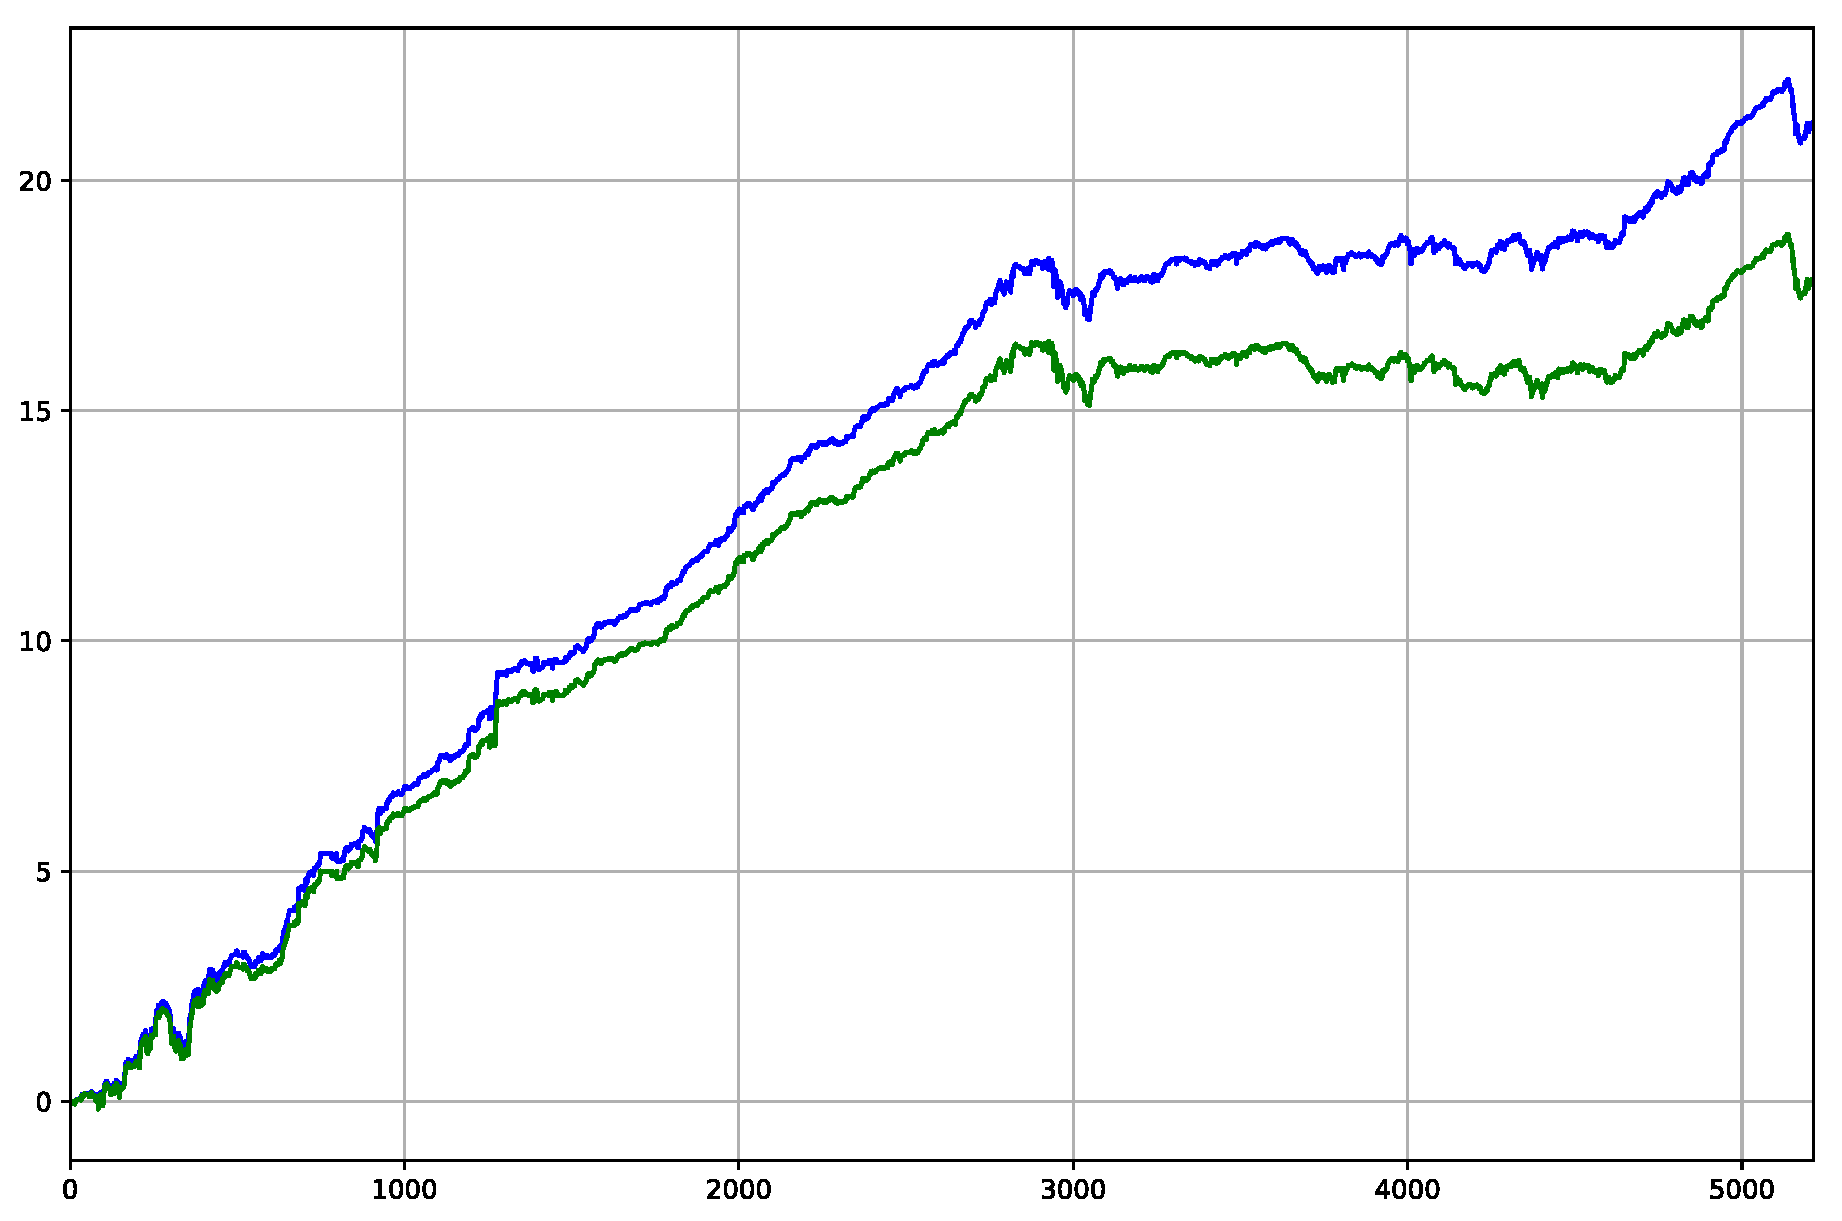
\includegraphics[width=\textwidth]{graphics/results2.pdf}
        \caption*{Rezultati simulacije na punom skupu dionica iz CROBEX-a.}
    \end{figure}}
    \only<2>{
      \begin{table}
        \centering
        \caption*{Rezultati simulacije na punom skupu dionica iz CROBEX-a.}
        \resizebox{0.8\textwidth}{!}{\begin{tabular}{lr}
            \toprule
            Rezultati: & \\
            \midrule
            bez troškova trgovanja: & \\
            ukupni profit & 24.32031 \\
            Sharpeov omjer &  2.16176 \\
            \midrule
            {uz uključene troškove trgovanja od 0.10\%:} & \\
            ukupni profit & 20.77131 \\
            Sharpeov omjer & 1.84749 \\
            \midrule
            prosječni koeficijent obrtaja & 0.68041\\
            prosječna konzistentnost & 0.81656 \\
            prosječna preciznost & 0.43558 \\
            \bottomrule
        \end{tabular}}
    \end{table}}
\end{frame}

  \section{Zaključak}
  \begin{frame}
    \frametitle{Zaključak}
    \begin{itemize}
      \item \textbf{poboljšanje} postojećih metoda statističke arbitraže
      \item algoritam radi \textbf{bolje} što je \textbf{više} vrijednosnica na raspolaganju
      \item algoritam radi \textbf{dobro} i uz isključenu mogućnost \emph{kratke pozicije}
      \item \textbf{nije otporan} na \emph{fundamentalni rizik}
    \end{itemize}
  \end{frame}

  \begin{frame}
    \frametitle{Hvala na pažnji!}
    \centering \Huge Pitanja?
\end{frame}
  
\end{document}